\documentclass[
%a4paper,12pt
encoding=utf8
]{../twoeskd}

% \usepackage{eskdappsheet}

% Packages required by doxygen
\usepackage[export]{adjustbox} % also loads graphicx
\usepackage[draft]{graphicx}
\usepackage[utf8]{inputenc}
\usepackage{multicol}
\usepackage{multirow}
\usepackage{makeidx}

% NLS support packages
\usepackage[T2A]{fontenc}
\usepackage[russian]{babel}
\usepackage{pscyr}

% Font selection
\usepackage{courier}
\usepackage{amssymb}

% Page & text layout
% \usepackage{geometry}
% \geometry{%
%   a4paper,%
%   top=2.5cm,%
%   bottom=4.5cm,%
%   left=2.5cm,%
%   right=2.5cm%
% }
%\setlength{\emergencystretch}{15pt}
\setlength{\parindent}{0cm}
\setlength{\parskip}{0.2cm}

% Headers & footers
% \usepackage{fancyhdr}
% \pagestyle{fancyplain}
% \fancyhead[L]{\fancyplain{}{}}
% \fancyhead[C]{\fancyplain{}{\scriptsize\textbf{RU.17701729.509000 ТЗ 01-1-ЛУ}}}
% \fancyhead[R]{\fancyplain{}{}}
% \fancyfoot[L]{\fancyplain{}{}}
% \fancyfoot[C]{\fancyplain{}{}}
% \fancyfoot[R]{\fancyplain{}{}}

% debug to see the frame borders
% from https://en.wikibooks.org/wiki/LaTeX/Page_Layout
% \usepackage{showframe}

% Indices & bibliography
\usepackage{natbib}
\usepackage[titles]{tocloft}
\setcounter{tocdepth}{3}
\setcounter{secnumdepth}{5}

% change style of titles in \section{}
\usepackage{titlesec}
\titleformat{\section}[hang]{\Large\bfseries\center}{\thetitle.}{1em}{}
\titleformat{\subsection}[hang]{\large\normalfont\raggedright}{\thetitle.}{1em}{\underline}
\titleformat{\subsubsection}[hang]{\normalsize\normalfont\raggedright}{\thetitle.}{1pt}{}

% Packages for text layout in normal mode
% \usepackage[parfill]{parskip} % автоматом делает пустые линии между параграфами, там где они есть в тексте
% \usepackage{indentfirst} % indent even in first paragraph
\usepackage{setspace}	 % controls space between lines
\setstretch{1} % space between lines
\setlength\parindent{0.9cm} % size of indent for every paragraph
\usepackage{csquotes}% превратить " " в красивые двойные кавычки
\MakeOuterQuote{"}


% this makes items spacing single-spaced in enumerations.
\newenvironment{my_enumerate}{
\begin{enumerate}
  \setlength{\itemsep}{1pt}
  \setlength{\parskip}{0pt}
  \setlength{\parsep}{0pt}}{\end{enumerate}
}


% Custom commands
% configure eskd
\titleTop{
\textbf{\Large ПРАВИТЕЛЬСТВО РОССИЙСКОЙ ФЕДЕРАЦИИ \\
НАЦИОНАЛЬНЫЙ ИССЛЕДОВАТЕЛЬСКИЙ УНИВЕРСИТЕТ \\
«ВЫСШАЯ ШКОЛА ЭКОНОМИКИ» } \\
\vspace*{0.2cm}
{\small Факультет компьютерных наук \\
Департамент программнoй инженерии \\
}
}
\titleDesignedBy{Студент группы БПИ 151 НИУ ВШЭ}{Абрамов А.M.}
\titleAgreedBy{%
\parbox[t]{7cm} {
Доцент департамента \\
программной инженерии \\
факультета компьютерных наук \\
канд. техн. наук \\
}}{Р. З. Ахметсафина}
\titleApprovedBy{
\parbox[t]{7cm} {
Академический руководитель \\
образовательной программы \\
«Программная инженерия» \\
профессор \\
канд. техн. наук \\
}}{В. В. Шилов}
\titleName{ПРОГРАММА СКЕЛЕТНАЯ АНИМАЦИЯ}
\workTypeId{RU.17701729.509000 T3 01-1-ЛУ}

\titleSubname{Программа и методика испытаний}

% Custom packages
\usepackage{pdfpages}

\makeindex

%===== C O N T E N T S =====


\begin{document}
% Titlepage & ToC
\pagenumbering{roman}

% some water filling text, that is pointless but adds text
% \newpage

\begin{center}
{\large АННОТАЦИЯ}
\end{center}

Настоящий документ представляет собой техническое задание для разработки приложения реализации алгоритма скелетной анимации. Данный документ составлен в соответствии с ГОСТ. В документе содержатся следующие разделы: «Введение», «Основания для разработки», «Назначение разработки», «Требования к программе», «Технико-экономические характеристики», «Стадии и этапы разработки», «Порядок контроля и приемки».

В разделе «Введение» содержится информация о намиеновании и краткой характеристике разрабатываемого приложения.

В разделе «Основания для разработки» содержится информация о документах, на основании которых ведется разработка настоящего приложения, а так же наименование темы разработки.

В разделе «Назначение разработки» содержится информация о функциональном и эксплуатационном назначении разрабатываемого прилоежния.

В разделе «Требования к программному изделию» содержится информация о требованиях к функциональным характеристикам, требованиях к надежности, условиях эксплуатации, требованиях к составу и параметрам технических средств, требования к информационной и программной совместимости.

В разделе «Требования к программной документации» содержится информация о требованиях, в соответствии с которыми должна выполняться разработка программной документации приложения.

В разделе «Технико-экономические показатели» содержится информация об ориентировочной экономической эффективности и ожидаемой годовой потребности, экономических преимуществах разработки по сравнению с лучшими зарубежными и отечественными аналогами.

В разделе «Стадии и этапы разработки» содержится информация о необходимых стадиях разработки, этапах и содержании работ. Присутствует информация о сроках разработки и исполнителях.

В разделе «Порядок контроля и приемки» содержится подробная информация о видах испытаний, которые будут применены к данному приложению, а так же общих требованиях к приемке работ.

Перед прочтением настоящего документа рекомендуется ознакомиться со списком терминов, для предотвращения непонятных моментов.



\newpage
\pagenumbering{arabic}
\tableofcontents
% \pagenumbering{arabic}

% --- add my custom headers ---
\newpage
\section{Объект испытаний}
\subsection{Наименование}
Наименование программы - "Программа скелетная анимация"

\subsection{Область применения}
"Программа скелетная анимация" - программа, позволяющая просмотреть файл описывающий анимацию в трехмерном пространстве. 

Программа является просмоторщиком файлов. В ее задачи входит чтение файла в определенном формате, рассчет параметров не записанных  в файле, но которые косвенно определяются по присутствующей информации, и наконец отображение этих данных на экране. 

Ее можно использовать для просмотра созданных художником 3-х мерных анимаций. 

Помимо формата файла, нобходимо понять какую именно информацию му хотим записывать в файл. 

В случае работы с алгоритмом скелетной анимации, в файл необходимо записать все вершины меша, "скелет" наложенный на данный меш и набор положений костей скелета в некоторые моменты времени.



\newpage
\section{Цель испытаний}
Цель проведения испытаний, - проверить, что разработанная программа соответствует требованиям к функциональности и надежности, изложенным в техническом задании к программе.


\newpage
\section{Требования к програмному изделию}


%=========================================
\subsection{Требования к функциональным характеристикам}
\subsubsection{Состав выполняемых функций}
\subsubsection{Организация входных и выходных данных}
\subsubsection{Прочие требования}


%=========================================
\subsection{Требования к временным характеристикам}
Требования к временным характеристикам программы не предъявляются.


%=========================================
\subsection{Требования к интерфейсу}
Интерфейс должен соответствовать схеме интерфейса, указанной в приложении.


%=========================================
\subsection{Требования к надежности}
\subsubsection{Обеспечение устойчивого функционирования программы}
Программа не должна вне зависимости от входных данных или действий оператора завершатся аварийно. При некорректно введенных параметрах пользователю должно отображаться сообщение об ошибке внутри окна ввода около поля (или группы полей), в которое(-ые) было введено некорректное значение.
\subsubsection{Время восстановления после отказа}
Требования к восстановлению после отказа не предъявляются.
\subsubsection{Отказы из-за некорректных действий оператора}
При попытке запуска алгоритма при не всех введенных данных или данных введенных некорректно, пользователю должно выдаваться сообщение в окне MessageBox.


%=========================================
\subsection{Требования к условиям эксплуатации}
\subsubsection{Климатические условия}
Условия соответствующие условиям эксплуатации современных компьютеров.
\subsubsection{Вид обслуживания}
Приложение не требует каких-либо видов обслуживания.
\subsubsection{Численность и квалификация персонала}
Минимальное количество персонала, требуемого для работы программы: 1 оператор. Пользователь программы должен знать следующие понятия из линейной алгебры, программирования и 3-х мерного моделирования: вектор, кватернион, матрица направляющих косинусов, меш (англ. mesh), коренная вершина (англ. root node).


%=========================================
\subsection{Требования к составу и параметрам технических средств}
Для оптимальной работы приложения необходимо учесть следующие системные требования:
\begin{my_enumerate}
\item Компьютер, оснащенный:
    \begin{my_enumerate}
    \item 32-разрядный (x86) или 64-разрядный (x64) процессор с тактовой частотой 1 гигагерц (ГГц) или выше;
    \item 512 мегабайт (ГБ) оперативной памяти (ОЗУ);
    \item 1 гигабайт (ГБ) (для 32-разрядной системы) или 2 ГБ (для 64-разрядной системы) пространства на жестком диске;
    \item графическое устройство OpenGL с драйвером версии 3.1 или выше.
    \item видеоадаптер super VGA с расширением 800*600 либо более высоким.
    \end{my_enumerate}
\item Монитор
\item Видеокарта
\item Мышь
\item Клавиатура
\end{my_enumerate}


%=========================================
\subsection{Требования к информационной и програмной совместимости}
Исходный код программы обязательно должен быть написан с использованием языка C\#. Приложению необходим компьютер с поддержкой OpenGL версии не менее 3.1. Операционная система Windows 7 или более поздняя версия Windows. Должен быть установлен .NET Framework версии не ниже 2.0.



\newpage
\section{Требования к програмной документации}
\subsection{Предварительный состав программной документации}
В обязательном порядке должны входить:
\begin{my_enumerate}
\item Техническое задание  (ГОСТ 19.201-78)
\item Пояснительная записка  (ГОСТ 19.404-79)
\item Руководство оператора  (ГОСТ 19.505-79)
\item Программа и методика испытаний (ГОСТ 19.301-79*)
\item Текст программы  (ГОСТ 19.401-78*)
\end{my_enumerate}



\newpage
\section{Средства и порядок испытаний}
%=========================================
\subsection{Параметру технических средств, используемых во время испытаний}
Для испытания программы необходимо учесть следующие системные требования:
\begin{my_enumerate}
\item Компьютер, оснащенный:
    \begin{my_enumerate}
    \item Обязательно 64-разрядный (x64) процессор с тактовой частотой 1 гигагерц (ГГц) или выше;
    \item 256 мегабайт (МБ) оперативной памяти (ОЗУ);
    \item 2 ГБ (для 64-разрядной системы) пространства на жестком диске;
    \item графическое устройство OpenGL с драйвером версии 3.1 или выше.
    \end{my_enumerate}
\item Монитор
\item Видеокарта
\item Мышь
\item Клавиатура
\end{my_enumerate}


%=========================================
\subsection{Программные средства, необходимые для проведения испытаний}
Приложению необходим компьютер с поддержкой OpenGL версии не менее 3.1. 64-битная операционная система Windows 7 или более поздняя версия Windows. Должен быть установлен .NET Framework версии не ниже 4.5.1, а также библиотеки Assimp версии не ниже 3.1 и OpenTK версии не ниже 1.1.4

%=========================================
\subsection{Порядок проведения испытаний}
Испытания должны проводиться в следующем порядке:
\begin{my_enumerate}
\item Проверка требований к документации.
\item Проверка требований к интерфейсу.
\item Проверка требований к функциональным возможностям программы.
\item Проверка требований надежности.
\end{my_enumerate}


%=========================================
\subsection{Условия проведения испытаний}

\subsubsection{Требования к численности и калификации персонала}
Для испытания программы требуется один оператор. Оператор программы должен иметь образование не ниже среднего общего и обладать базовыми знаниями следующих понятий из линейной алгебры, программирования и трехмерного моделирования: вектор, кватернион, матрица направляющих косинусов, меш (англ. mesh), кость, корневая вершина (англ. root node).






\newpage
\section{Методы испытаний}
Испытания представляют собой процесс установления соответствия программы и
программной документации заданным требованиям.

\subsubsection{Проверка требований к документации}
Проверяеться наличие всех документов перечисленных в пyнкте 4.1 данного документа и их соответствие ГОСТ.

\subsection{Проверка требований к интерфейсу}
Интерфейс соответствует схеме, указанной в техническом задании, обладает шкалой времени, панелью для отображения иерархии, панелью для изменения настроек программы и панелью для отрисовки трехмерных элементов.

\begin{figure}[h!]
    \centering
    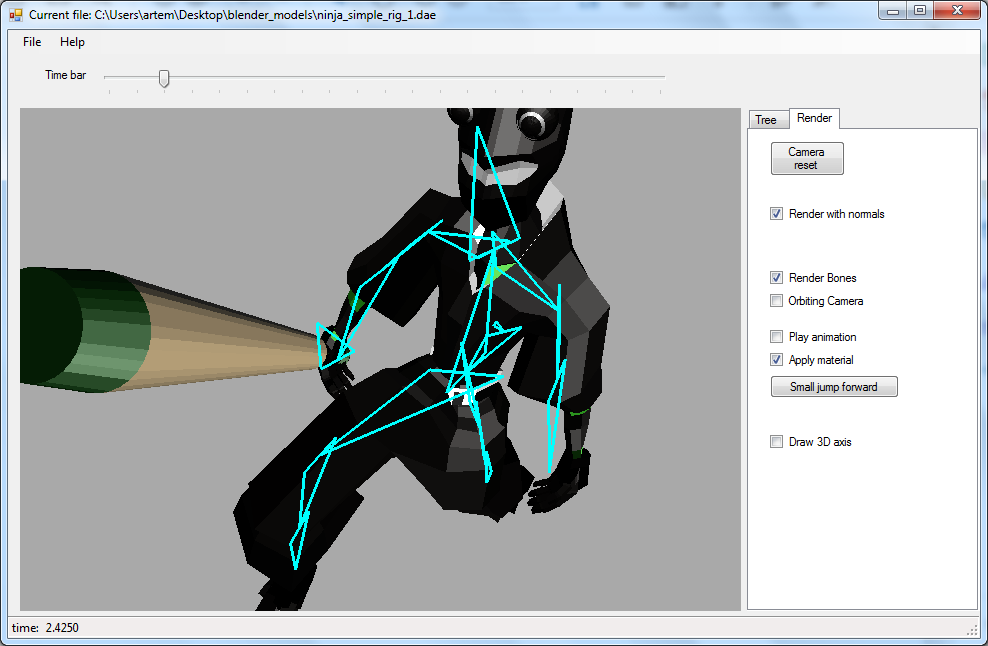
\includegraphics[width=0.5\textwidth]{../screenshots/interface_map.png}
    \caption{Изображение интерфейса программы}
\end{figure}

Дополние панели также удовлетворяют требованиям ТЗ:
\begin{figure}
\centering
\begin{minipage}{.4\textwidth}
  \centering
  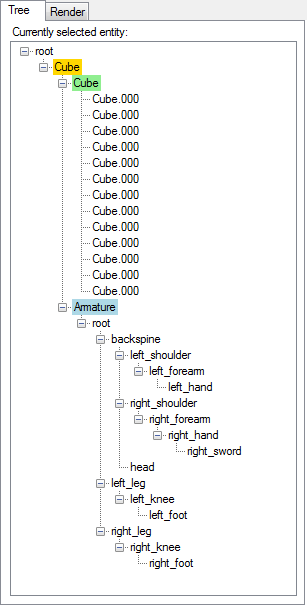
\includegraphics[height=.2\textheight]{../screenshots/tree_view_panel.png}
  \captionof{figure}{Панель отображения иерархии костей}
\end{minipage}%
\begin{minipage}{.4\textwidth}
  \centering
  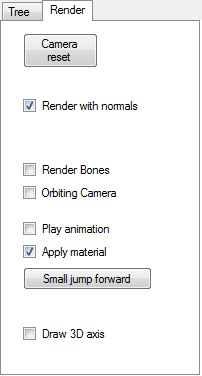
\includegraphics[height=.2\textheight]{../screenshots/render_panel.png}
  \captionof{figure}{Панель настройки программы}
\end{minipage}
\end{figure}

\subsection{Проверка требований к функциональным характеристикам}
Для загрузки данных из формата коллада (collada или .dae) необходимо выбрать его либо в меню "Open Recent", либо в меню "Open":

\begin{figure}[h!]
    \centering
    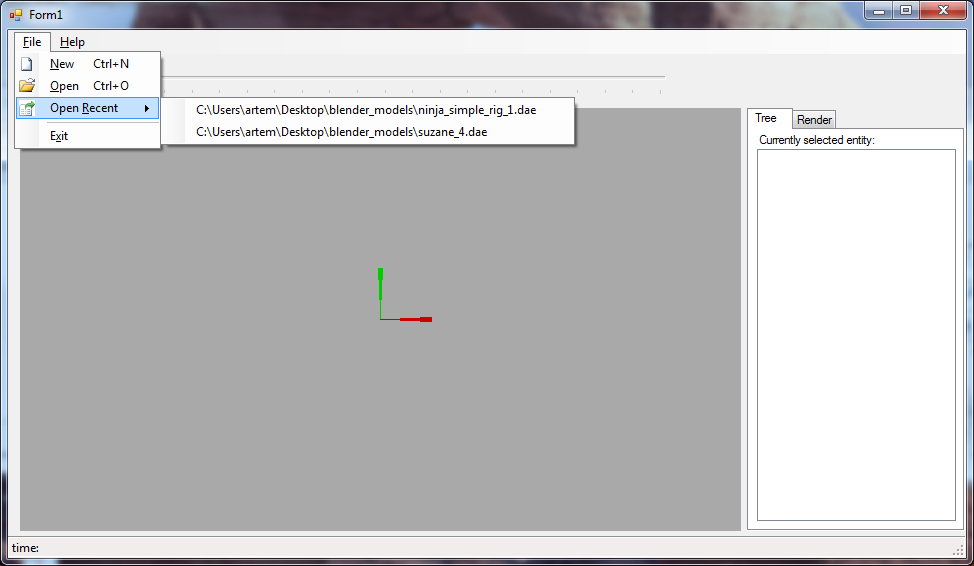
\includegraphics[width=0.8\textwidth]{../screenshots/file_menu_with_recent.png}
    \caption{Загрузка файла}
\end{figure}

Откроется диалог выбора файла:
\begin{figure}[h!]
    \centering
    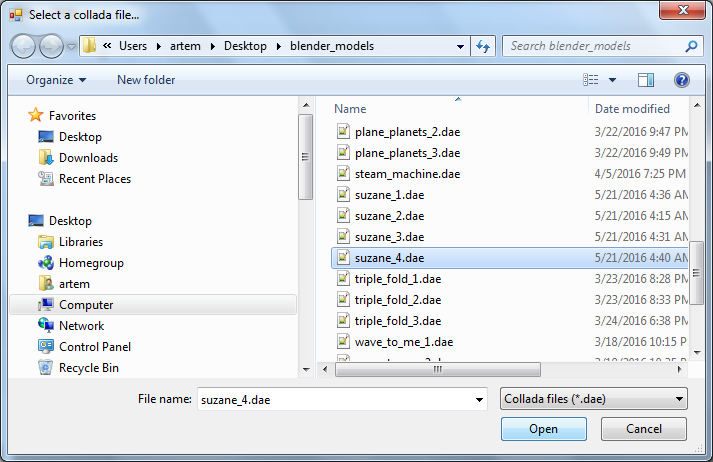
\includegraphics[width=0.5\textwidth]{../screenshots/open_file_dialog.png}
    \caption{Диалог выбора файла}
\end{figure}

После загрузки файла видно что его имя добавилось в список недавно открытых файлов "Recent Files".


%=================
У пользователя имеется возможность изменять ракурс и приближение камеры при помощи мышки. Структура загруженных данных отображена в виде дерева на панели справа. Также выделенная кость подсвеченна ярко-синим цветом.

\begin{figure}[h!]
    \centering
    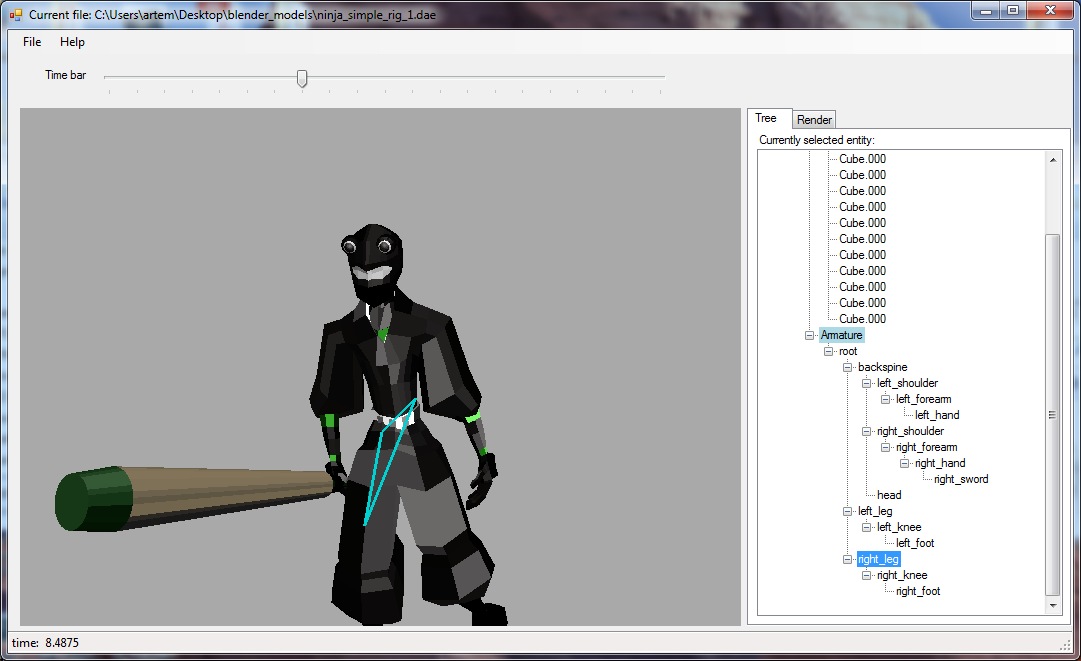
\includegraphics[width=0.8\textwidth]{../screenshots/frame_with_one_bone.png}
    \caption{Подсветка выбранной кости}
\end{figure}

Также есть панель для настоек работы программы позволяющая изменять следующие параметры:
\begin{my_enumerate}
\item Выбор между двумя видами камер в OpenGL, первый вид это камера движение которой сковано орбитой вокруг модели и другой тип это камера двигающаяся совершенно свободно.
\item Воспроизведение анимации.
\item Включение и выключение отрисовки с учетом нормалей.
\item Включение и выключение отрисовки с учетом характеристик материала.
\item Отрисовка всех костей скелета.
\end{my_enumerate}

%=================
Элемент ScrollBar показывает текущий момент в анимации и предоставляет 
возможность перейти к любому моменту времени. 

\begin{figure}[h!]
    \centering
    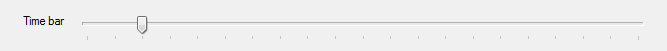
\includegraphics[width=0.5\textwidth]{../screenshots/time_bar.png}
    \caption{Элемент ScrollBar}
\end{figure}

\bigskip

Поддерживатся изменение размеров окна приложения, без изменения соотношения проекции OpenGL.


\subsection{Проверка требований к надежности}
Оператор должен воспользоваться всеми функциями программы и убедиться, что они не приводят к ее аварийному завершению.


\newpage
\section{Приложение 1. Терминология}
\subsection{Терминология}
\begin{description}

\item[Корневая вершина (англ. root node)]  
Самый верхний узел дерева.

\item[Полигональная сетка (жарг. меш от англ. polygon mesh)]
Совокупность вершин, рёбер и граней, которые определяют форму многогранного объекта в трехмерной компьютерной графике и объёмном моделировании. Гранями являются треугольники.

\item[Дерево]
Связный ациклический граф. Связность означает наличие путей между любой парой вершин, ацикличность — отсутствие циклов и то, что между парами вершин имеется только по одному пути.

\item[Степень вершины]
Количество инцидентных ей (входящих/исходящих из нее) ребер.

\item[Интерполяция, интерполирование анимации]
Способ нахождения промежуточных значений состояния анимации по имеющемуся дискретному набору известных значений.

\item[Z-буферизация]
В компьютерной трёхмерной графике способ учёта удалённости элемента изображения. Представляет собой один из вариантов решения «проблемы видимости»

\item[Z-конфликт (англ. Z–fighting)]
Если два объекта имеют близкую Z-координату, иногда, в зависимости от точки обзора, показывается то один, то другой, то оба полосатым узором.

\item[OpenGL (Open Graphics Library)]
Спецификация, определяющая независимый от языка программирования платформонезависимый программный интерфейс для написания приложений, использующих двумерную и трёхмерную компьютерную графику. На платформе Windows конкурирует с Direct3D.

\item[Рендеринг (англ. rendering — «визуализация»)]
Термин в компьютерной графике, обозначающий процесс получения изображения по модели с помощью компьютерной программы.

\item[Текстура]
Растровое изображение, накладываемое на поверхность полигональной модели для придания ей цвета, окраски или иллюзии рельефа. Приблизительно использование текстур можно легко представить как рисунок на поверхности скульптурного изображения.

\end{description}



\newpage
\section{Приложение 2. Список используемой литературы}
\subsection{Список используемой литературы}
\begin{my_enumerate}
\item
OpenGL Superbible: Comprehensive Tutorial and Reference (7th Edition)
Graham Sellers (Author), Richard S Wright Jr. (Author), Nicholas Haemel (Author)
ISBN-13: 978-0672337475

\item
Порев В.Н. Компьютерная графика. – СПб.: БХВ-Петербург, 2002. – 432 с.: ил.

\item
ГОСТ 19.102-77 Стадии разработки. //Единая система программной документации. -М.: ИПК Издательство стандартов, 2001.

\item
ГОСТ 19.201-78 Техническое задание. Требования к содержанию и оформлению // Единая система программной документации. -М.:ИПК Издательство стандартов, 2001.

\item
ГОСТ 19.101-77 Виды программ и программных документов
//Единая система программной документации. -М.: ИПК Издательство стандартов, 2.: 001.

\item
ГОСТ 19.103-77 Обозначения программ и программных документов. //Единая система программной документации. -М.: ИПК Издательство стандартов, 2001.

\item
ГОСТ 19.104-78 Основные надписи //Единая система программной документации. -М.: ИПК Издательство стандартов, 2001.

\item 
ГОСТ 19.105-78 Общие требования к программным документам. //Единая система
программной документации. – М.: ИПК Издательство стандартов, 2001.

\end{my_enumerate}



% \newpage
%\section{Приложение 3. Изображение пользовательского интерфейса.}

% Index
\newpage
\eskdListOfChanges

% \phantomsection
% \addcontentsline{toc}{section}{Алфавитный указатель}
% \printindex

\end{document}
